\documentclass{article}
\usepackage{graphicx}
\usepackage[utf8]{ctex}
\usepackage{amsmath}
\usepackage[fontsize=10pt]{fontsize}
\usepackage{geometry}
\geometry{a4paper,left=0.75in,right=0.75in,top=1in,bottom=0.75in}
\usepackage{setspace}
\setlength{\parindent}{0em}
\def\kong{\hspace*{2em}}
\usepackage{amsfonts,amssymb}
\usepackage{xcolor}
\usepackage{fontspec}
\usepackage{enumitem}
\linespread{1.5}
\usepackage{hyperref}
\usepackage{hyperref}
\hypersetup{hidelinks,
	colorlinks=true,
	allcolors=black,
	pdfstartview=Fit,
	breaklinks=true}

\usepackage{listings}
	\lstset{
 columns=fixed,
 numbers=left,
 numberstyle=\tiny\color{gray},
 frame=none,
 backgroundcolor=\color[RGB]{245,245,244},
 keywordstyle=\color[RGB]{40,40,255},
 numberstyle=\footnotesize\color{darkgray},
 commentstyle=\it\color[RGB]{0,96,96},
 stringstyle=\rmfamily\slshape\color[RGB]{128,0,0},
 showstringspaces=false,
 language=c,
 basicstyle=\ttfamily
	}

\usepackage{fancyhdr}

\pagestyle{fancy}
\fancyhf{}
\fancyhead[LE,RO]{\thepage}
\fancyhead[RE,LO]{\kaishu PB21000276施耀炜}



\date{2022年3月}

\begin{document}

\setcounter{page}{1}
\thispagestyle{empty}
\kong
\\[10pt]
\begin{center}
	\textbf{\huge \heiti 实验报告二}\\[6pt]
    \textbf{\huge \heiti 硅光电池特性的研究}\\[12pt]
	\textbf{学号：}\underline{\kaishu PB21000276} \qquad 
    \textbf{姓名：}\underline{\kaishu 施耀炜} \qquad 
    \textbf{班级：}\underline{\kaishu 21级少院6班}\qquad 
    \textbf{日期：}\underline{2022年3月23日}\\[24pt]
\end{center}
\section{实验名称}
    \kong 硅光电池特性的研究
\section{实验目的}
    \kong 了解硅光电池工作原理，掌握硅光电池的工作特性。
\section{实验原理}
    \kong 硅光电池是根据光伏效应而制成的将光能转换成电能的一种器件。
    \subsection{P-N结特性}
        \kong 空穴较多的P型半导体和电子较多的N型半导体结合时，
        空穴从P向N扩散，电子从N向P扩散，中间形成的耗散区即离子层
        无自由载流子，有稳定的内电场，呈现高抗阻，即P-N结。
        因此其具有单向导电性的特点，正偏时导通，反偏时耗尽区变宽。
    \subsection{光伏效应}
        \kong P-N结处于零偏或反偏时，耗尽区存在内电场，有光照时，
        电池对光子的本征吸收所激发的少数载流子引起光伏效应。
        激发出的电子空穴对在内电场作用下分别飘 移到 N 型区和 P 型区，
        当在 PN 结两端加负载时就有一光生电流流过负载，此即光伏效应。
    \subsection{硅光电池的基本特性}
        \subsubsection{伏安特性}
            \kong 一定光照下，光电池两端加负载就会有电流流过，
            负载很大时，电流较小而电压较大;
            负载很小时，电流较大而电压较小。
            硅光电池的伏安特性曲线由二个部分组成: 
            无偏压工作状态，光电流随负载变化很大；
            反偏压工作状态，光电流与偏压、负载几乎无关(很大动态范围内)。
        \subsubsection{照度特性}
            \kong 当没有光照时，硅光电池等效于普通的二极管，其伏安特性为：
            \[
                I_{d}=I_{0}\left[\exp \left(\frac{q U}{k_{B} T}\right)-1\right] \eqno{(2.1)}
            \]
            $I_d$ 为流过 PN 结的电流，$I_0$ 为反向饱和电流，
            $q$ 为电子电荷，$k_B$ 为玻尔兹曼常数，
            $T$ 为绝对温度，$U$ 是 加在 P-N 结两端电压。
            对于外加正向电压， $I_d$ 随$V$ 指数增长，称正向电流；
            当外加电压为反向时，在反向击穿电压之内，
            反向饱和电流基本是个常数。\\
            \kong 当有光照时，
            激发出的电子空穴对在内电场作用下分别飘逸到 N 型区和 P 型区，
            当在 PN 结两端加负载时就有光生电流流过负载，
            流过 PN 结两端的电流：
            \[
                I=I_{p h}-I_{0}\left[\exp \left(\frac{q U}{k_{B} T}\right)-1\right] \eqno{(2.2)}
            \]
            $I_{ph}$ 是与入射光的强度成正比的光生电流，
            与负载电阻大小及硅光电池结构特性有关。
        \subsubsection{输出特性}
            \kong 硅光电池负载$R_L$上的电压降$U$和通过$R_L$的电流之积
            称为硅光电池的输出功率$P$。
            输出功率达到最大值$P_m=U_mI_m$时的负载电阻$R_m$称为最佳负载电阻，
            此时能量转换效率最高，且$R_m$随光强而变化。
            定义填充因子$FF$：
            \[
                F F \equiv \frac{P_{m}}{U_{o c} I_{S C}}=\frac{U_{m} I_{\mathrm{m}}}{U_{o c} I_{S C}} \eqno{(2.3)}
            \]
            是表征硅光电池性能优劣的重要参数，
            取决于入射光强、材料禁带宽度、负载电阻等。
%实验仪器
\section{实验仪器}
    \begin{itemize}[noitemsep]
        \item 硅光电池
        \item 数字万用表
        \item 毫安表
        \item 电阻箱
        \item 溴钨灯
        \item 直流稳压电源
        \item 光学导轨及支座
        \item 开关
        \item 导线
    \end{itemize}
%数据处理与分析
\newpage
\section{数据处理与分析}
    \subsection{硅光电池暗伏安特性测量}
        \kong 在全黑条件下，测量硅光电池正向偏压时伏安特性曲线。
        下面是本实验的原始数据，电流表使用$20\text{mA}$量程，万用表选择$2\text{V}$量程。
        \begin{figure}[htp]
            \centering
            \textbf{表\ 2.1}\quad 暗伏安特性原始数据\\[4pt]
            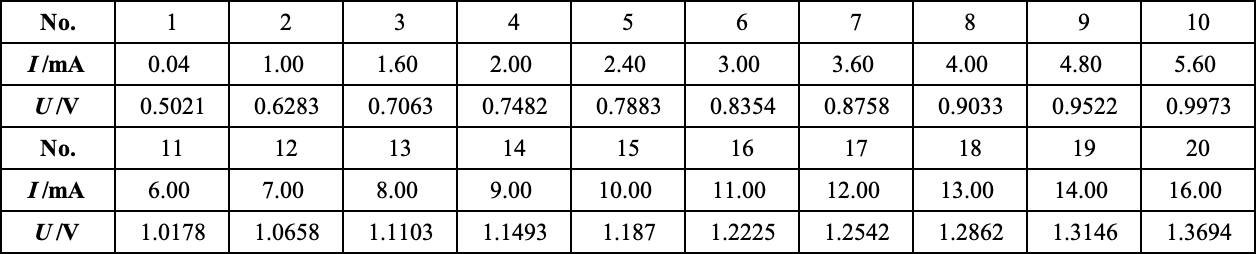
\includegraphics[width=13.2cm]{bg1.png}
        \end{figure} 
        得伏安曲线如下：
        \begin{figure}[htp]
            \centering
            \textbf{图\ 2.1}\quad 暗伏安特性曲线\\
            
\includegraphics[width=14cm]{tp3.png}
        \end{figure} 
    \newpage
    \subsection{硅光电池输出特性测量}
        \kong 用溴钨灯照射硅光电池，电阻箱为负载，测量不同$L$、$R_L$下硅光电池的工作电压$U$，
        求出工作电流$I$和功率$Р$，绘制$I-U$、$P-R_L$曲线。
        原始数据及所计算的$I$、$P$、$L$在表2.2中列出。得$I-U$、$P-R_L$曲线，于图2.2、图2.3所示。\\
        \kong 其中$R_L=50\Omega$时使用$200\text{mV}$量程，其余使用$2\text{V}$量程。
        \begin{figure}[htp]
            \centering
            \textbf{表\ 2.2}\quad 输出特性数据\\[4pt]
            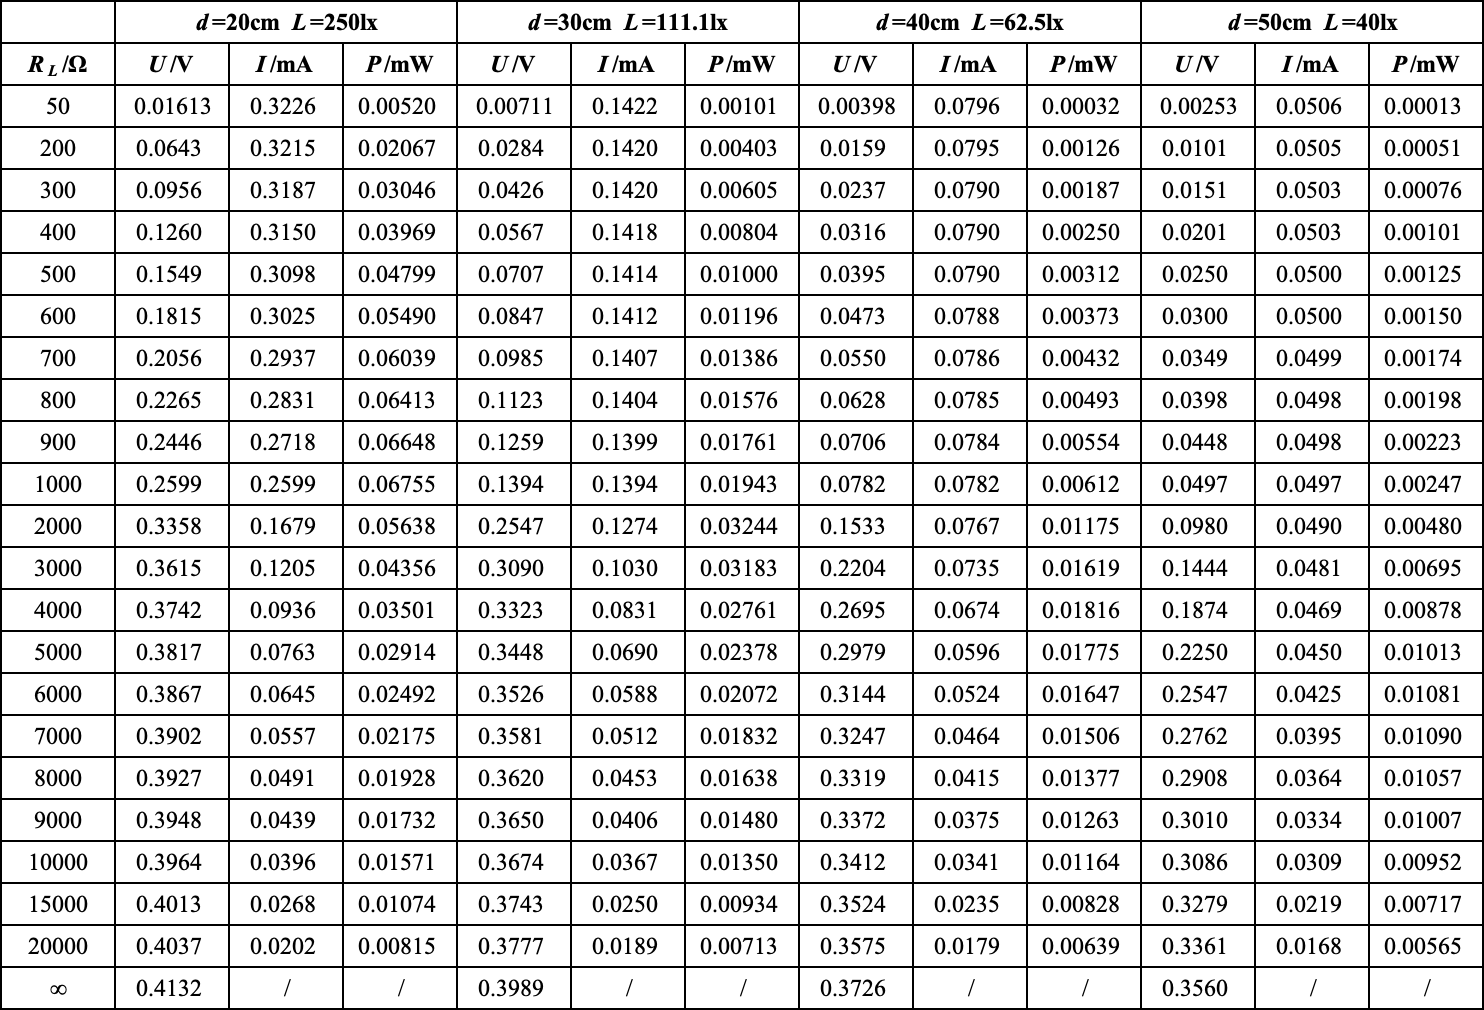
\includegraphics[width=15.6cm]{bg2.png}
        \end{figure}
        \begin{figure}[htp]
            \centering
            \textbf{图\ 2.2}\quad 输出特性$I-U$曲线\\
            
\includegraphics[width=14cm]{tp1.png}
        \end{figure} 
        \begin{figure}[htp]
            \centering
            \textbf{图\ 2.3}\quad 输出特性$P-R_L$曲线\\
            
\includegraphics[width=14cm]{tp2.png}
        \end{figure}
    \newpage
    \subsection{硅光电池开路电压与短路电流测量}
        \kong 测量不同光照下硅光电池的开路电压 $U_{oc}$、
        短路电流 $I_{SC}$，绘制 $U_{oc}-L$、$I_{SC}-L$ 曲线，
        短路电流用负载$R_L=50\Omega $时得电流代替，数据如表2.3所示，
        得$U_{oc}-L$、$I_{SC}-L$ 曲线，分别于图2.4、图2.5所示。\\
        \kong 其中$R=50\Omega$时使用$200\text{mV}$量程，开路电压使用$2\text{V}$量程。
        \begin{figure}[htp]
            \centering
            \textbf{表\ 2.3}\quad 开路电压与短路电流数据\\[4pt]
            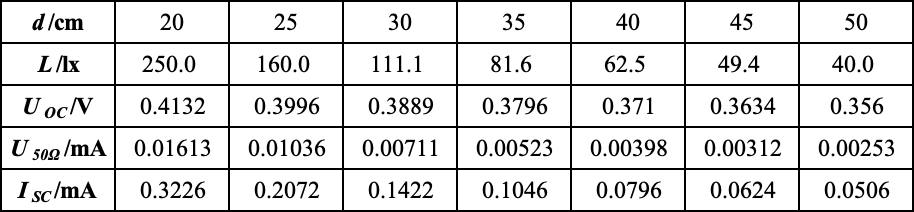
\includegraphics[width=9.6cm]{bg3.png}
        \end{figure}
        \begin{figure}[htp]
            \centering
            \textbf{图\ 2.4}\quad $U_{oc}-L$曲线\\
            
\includegraphics[width=14cm]{tp4.png}
        \end{figure} 
        \newpage
        \begin{figure}[htp]
            \centering
            \textbf{图\ 2.5}\quad $I_{SC}-L$曲线\\
            
\includegraphics[width=14cm]{tp5.png}
        \end{figure}
        $I_{SC}-L$曲线表明，硅光电池的短路电流在一定范围内和光照度的关系很接近正比.
    \newpage 
    \subsection{不同负载下硅光电池输出电压与光照测量}
        \kong 测量不同负载 $R_L$ 的硅光电池输出电压 $U$ 与光照度 $L$ 的关系，绘制 $U-L$ 曲线并分析负载对 $U-L$ 的
        影响。原始数据如表2.4所示，得 $U-L$ 曲线如图2.6所示。\\
        \kong 其中$R_L=100\Omega$时使用$200\text{mV}$量程，其余使用$2\text{V}$量程。
        \begin{figure}[htp]
            \centering
            \textbf{表\ 2.3}\quad 不同负载的输出电压数据\\[4pt]
            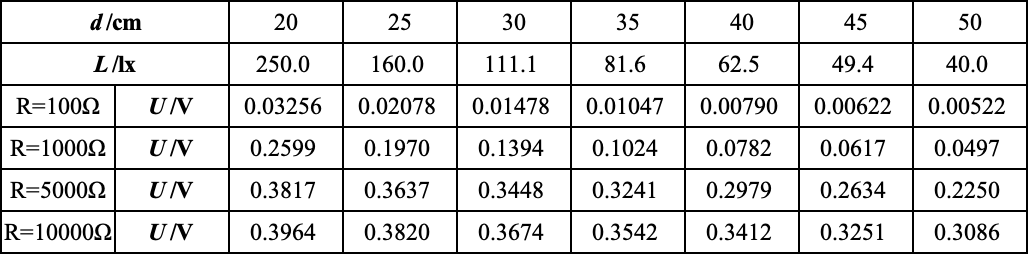
\includegraphics[width=10.8cm]{bg4.png}
        \end{figure}
        \begin{figure}[htp]
            \centering
            \textbf{图\ 2.6}\quad 不同负载下的$U-L$曲线\\
            
\includegraphics[width=14cm]{tp6.png}
        \end{figure}
        \\可以看到，负载越大，在同一光照度下硅光电池的输出电压也越大。
        而且当负载越小时，负载变化对输出电压的变化影响越大。
\newpage
\section{分析与讨论}
    \subsection{定性误差分析}
    \kong \textbf{1.}光照度：\\
    \kong \kong (1)光源的亮度可能因为电压电流等的变化而有所波动；\\
    \kong \kong (2)实验仪器的上硅光电池所在的立柱并无中心刻度，可能导致距离$d$不准确；\\
    \kong \kong (3)导轨与电源前端、硅光电池与光线均可能不垂直；\\
    \kong \kong (4)环境中除了实验光源外的其他光源影响。\\
    \kong \textbf{2.}电流、电压：\\
    \kong \kong (1)电压表使用的是万用表，精度不足；\\
    \kong \kong (2)用$R_L=50\Omega$时的电流代替短路电流并不准确；\\
    \kong \kong (3)暗伏安特性测量时为电流表外接法，电流偏大。\\
    \kong \textbf{3.}电阻：\\
    \kong \kong (1)测量中发现存在“$1000\Omega \times10$”和“$10000\Omega$”
    电压不同的情况，电阻箱可能带来误差；\\
    \kong \kong (2)导线、接线柱等电阻的影响。
\section{思考题}
    \kong \textbf{1.}光电池在工作时为什么要处于零偏或反偏？\\
    \kong \textbf{答：}只有当P-N结处于零偏或反偏时，耗尽区才会存在内电场，
    此时对其光照，硅光电池对光子的本征吸收所激发的少数载流子才会引起光伏效应，
    即硅光电池正常工作；若正偏，则P-N结导通，此时耗尽区变窄，扩散运动大于飘逸运动，
    硅光电池便无法正常工作输出电压。\\
    \kong \textbf{2.}增加光照强度，硅光电池那些参数会发生变化？\\
    \kong \textbf{答：}增加光照强度会直接导致短路电流$I_{SC}$、
    断路电压$U_{oc}$、一定负载下的输出电压$U_L$、电流$I$、
    光生电流$I_{ph}$均增大，同时输出功率$P$也会改变。\\
\end{document}
